%
%
%
% Group addresses by affiliation; use superscriptaddress for long
% author lists, or if there are many overlapping affiliations.
% For Phys. Rev. appearance, change preprint to twocolumn.
% Choose pra, prb, prc, prd, pre, prl, prstab, prstper, or rmp for journal
%  Add 'draft' option to mark overfull boxes with black boxes
%  Add 'showkeys' option to make keywords appear
\documentclass[aps,pra,reprint, onecolumn]{revtex4-2}
% showkey for keywords
%\documentclass[aps,pra,reprint]{revtex4-2}
\usepackage{lipsum}
\usepackage{listings}
\usepackage{xcolor}

\definecolor{codegreen}{rgb}{0,0.6,0}
\definecolor{codegray}{rgb}{0.5,0.5,0.5}
\definecolor{codepurple}{rgb}{0.58,0,0.82}
\definecolor{backcolour}{rgb}{0.95,0.95,0.92}

\lstdefinestyle{pystyle}{
    commentstyle=\color{codegreen},
    keywordstyle=\color{magenta},
    numberstyle=\tiny\color{codegray},
    stringstyle=\color{codepurple},
    basicstyle=\ttfamily\footnotesize,
    breakatwhitespace=false,
    breaklines=true,
    captionpos=b,
    keepspaces=true,
    numbers=left,
    numbersep=5pt,
    showspaces=false,
    showstringspaces=false,
    showtabs=false,
    tabsize=2
}
\lstset{style=pystyle}

\usepackage{booktabs}
\usepackage{siunitx}
\usepackage{adjustbox}
\usepackage{tabularx}
\newcommand\setrow[1]{\gdef\rowmac{#1}#1\ignorespaces}
\newcommand\clearrow{\global\let\rowmac\relax}
\clearrow

\newcommand{\red}[1]{\textcolor{red}{#1}}
\newcommand{\blue}[1]{\textcolor{blue}{\textbf{figure: #1}}}
\newcommand{\teal}[1]{\textcolor{teal}{\textbf{equation: #1}}}
\newcommand{\purple}[3]{\textcolor{purple}{\textbf{\textit{#1}, #2, #3}}}

%\renewcommand{\subsubsection}[1]{\subsubsection{\textbf{#1}}}

\usepackage{amsmath}
\PassOptionsToPackage{hyphens}{url}\usepackage{hyperref}


\begin{document}

% Title of paper
\title{Quantum Walks with Time-Dependent Hamiltonian}
%\\ \small{Systematic comparison between time-independent and time-dependent \\ hamiltonian approach to quantum search}

% repeat the \author .. \affiliation  etc. as needed
% \email, \thanks, \homepage, \altaffiliation all apply to the current
% author. Explanatory text should go in the []'s, actual e-mail
% address or url should go in the {}'s for \email and \homepage.
% Please use the appropriate macro foreach each type of information

% \affiliation command applies to all authors since the last
% \affiliation command. The \affiliation command should follow the
% other information
% \affiliation can be followed by \email, \homepage, \thanks as well.
\author{Matteo Garbellini}
%\email[]{matteo.garbellini@studenti.unimi.it}
%\homepage[]{Your web page}
%\thanks{}
%\altaffiliation{}
\affiliation{Department of Physics \\ Universit\`a degli Studi di Milano \\ }

%Collaboration name if desired (requires use of superscriptaddress
%option in \documentclass). \noaffiliation is required (may also be
%used with the \author command).
%\collaboration can be followed by \email, \homepage, \thanks as well.
%\collaboration{}
%\noaffiliation

\date{\today}

%\begin{abstract}
%We introduce a novel algorithm for quantum search based on an dynamical implementation of the traditional laplacian hamiltonian, taking advantages of the adiabatic theorem and its implication. We then study the worst case scenario of a simple N-dimensional ring, which gives great localization results but poor time-optimized search results. We then apply the same method to the complete graph, trying to improve the standard continous quantum-walk Grover algorithm. Different time stepping functions are investigated, hopefully giving some useful insight on the dynamic of the constructed hamiltonian.
%\end{abstract}

% insert suggested keywords - APS authors don't need to do this
%\keywords{Quantum Search, Quantum Walk, Adiabatic Theorem}

%\maketitle must follow title, authors, abstract, and keywords
\maketitle

% body of paper here - Use proper section commands
% References should be done using the \cite, \ref, and \label commands

\red{I testi in rosso sono commenti su argomenti mancanti, informazioni da aggiungere e analisi necessarie per completare il lavoro. Una lista piu o meno completa si trova nella Sezione V. Una versione di questo report aggiornata volta per volta si puo trovare qui}\\ {\footnotesize \url{https://github.com/matteogarbellini/Quantum-Walk-Time-Dependent-Hamiltonian/blob/AdiabaticQuantumWalk/0.%20report/thesis_report.pdf}}

% % % % % % % % %
% INTRODUCTION  %
% % % % % % % % %
\section{Introduction}
This report can be summarized as follows.
\begin{itemize}
\item In Section II a review of the background topics is presented, with particular enphasis on Quantum Walks, Quantum Search and the Adiabatic Theorem. A brief introduction on Graph Theory is presented as well, in order to define the working context.
\item In Section III we discuss the Dynamics, focusing on the time dependent and time independent hamiltonian approach to quantum search. A definition of the computational routines used throughout the work is also given.
\item In Section IV we present results for selected topologies, namely the \textit{worst-case-scenario} Circular Graph and the \textit{best-case-scenario} Complete Graph. For the two selected topologies we compare the known time-independent approach and the time-dependent, in particular defining two qualitative characteristics for results: optimized search and localization.
\item Section V is a list of things yet to be done/finished.
\item In the Appendix a discussion on the computational methods, in particular the differential equation solver and the optimization algorithm used.
\end{itemize}

%%%%%%%
%BACKGROUND
%%%%%%%
\section{Background}

\subsection{Graph Theory}
A graph G is defined as a ordered pair $(V,E)$, where V is a set of vertices and E is a set of edges, which represent the connection between any two pair of vertices. If indeed any two vertices $(i,j)$ are connected by an edge we define as adjacent, and from this we can construct the \textit{adjacency matrix} A as:
\begin{equation}
A_{ij} = \begin{cases} 1 & (i,j)\in G \\ 0 & \mbox{otherwise} \end{cases}
\end{equation}
which represents the connectivity of the graph. We can then describe the degree of each vertex of the graph, namely the number of vertices (excluding itself) connected to it, through the \textit{degree diagonal matrix} $D_{jj} = deg(j)$.\\
It is also useful to introduce the \textit{laplacian matrix} defined as
\begin{equation}
  L = A-D
\end{equation}
which we'll later see describes the quantum walk evolution.\\
In the quantum realm a vertex is a vector in an N dimensional Hilber space, so that a vertex $|j\rangle$ can be represented in the following way
\begin{equation}
  |j\rangle = \begin{pmatrix} 1 \\ 0 \\ 0 \\ .. \\0 \end{pmatrix}
\end{equation}

Throughout this work we focus our attention on two particular graph topologies: the \textbf{circular} graph and the \textbf{complete} graph (FIG. 1).


\begin{figure}[ht]
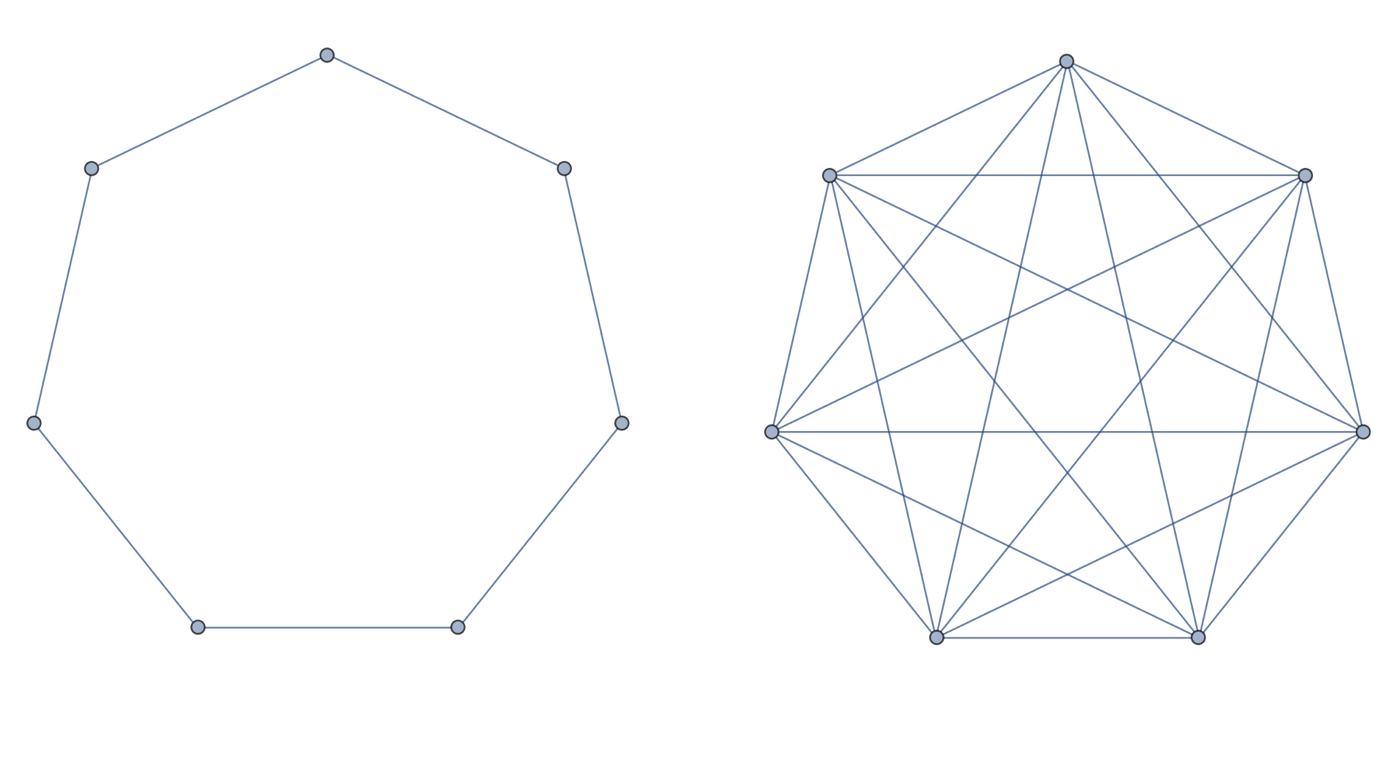
\includegraphics[width=9.5cm]{./figures/graph.png}%
\caption{Pictorial representation of a circular graph (left) and a complete graph (right) with N=7}
\end{figure}

\subsection{Quantum Walks}
The continous time quantum walk is the direct analougue of the classical random walk. Given a graph G, a random walk is a Markov process with a fixed probability for unit time $\gamma$ of jumping to an adjacent vertex $j$. This particular walk can be described by a linear differential equation in terms of probability, namely

\begin{equation}
  \frac{d}{dt}p_j(t) = \gamma\sum_{k}L_{jk}p_k(t)
\end{equation}

where $p_j(t)$ is the probability of being on the vertex $j$ at time $t$.\\
The quantum analogue takes place in an N-dimentional Hilbert space spanned by the states (vertex) $|j\rangle$ of the graph G. Instead of considering the classical probability as we previosuly did, we consider the probability time-dependent amplitudes $q_j(t) = \langle j|\psi(t)\rangle$, where $|\psi\rangle$ is a general time-dependent state. The differential equation takes thus the form of

\begin{equation}
  i\frac{d}{dt}q_j(t) = \sum_{k}H_{jk}q_k(t)
\end{equation}
The continous-time quantum walk is defined by letting $H=-\gamma L$, where $L$ is the previosuly defined Laplacian matrix.

\subsection{Grover's Quantum Search}
\red{This section should include the standard Grover's Quantum Search to give the contex for the quantum walk approach.}

\subsection{Quantum Search with Continous-Time Quantum Walk}
\purple{Spatial Search by Quantum Walk}{A. Childs, J. Goldstone}{quant-ph/0306054v2}\\
We now address the quantum search problem firstly formulated as Grover's algorithm and then extending it to the search on a graph using quantum walks. \\
To approach the Grover problem with quantum walk it's necessary to modify the hamiltonian such that the vertex $|w\rangle$, i.e. the target, is somewhat special. Following Grover's oracle an oracle hamiltonian $H_w$ is introduced

\begin{equation}
  H_w = -|w\rangle\langle w|
\end{equation}

which in particular has energy zero for all but the vertex $|w\rangle$ for which it has enenergy $-1$. Therefore the Grover problem, i.e. quantum search, becomes finding the ground state of such hamiltonian. To do so we consider the time-independent hamiltonian of the form
\begin{equation}
  H = -\gamma L + H_w = -\gamma L -|w\rangle\langle w|
\end{equation}
where L is the laplacian of the graph, which contains the information of the dynamics over that particular graph topology. The evolution of the quantum walk is therefore governed by this hamiltonian.\\

The quantum search routine works as follow:
\begin{itemize}
  \item we consider the superposition of all possible states, namely
  \begin{equation}
    |s\rangle = \frac{1}{\sqrt{N}}\sum_j|j\rangle
  \end{equation}

  \item we find the evolved state using the hamiltonian for a time T $H$
  \begin{equation}
  |\psi(T)\rangle = U(T)|s\rangle  = \mbox{exp}\Big\{-\frac{i}{\hbar}HT\big\}|s\rangle
  \end{equation}
  (Note that this evolution is valid only for time-independent hamiltonians.)

  \item we then measure the state onto the target $|w\rangle$ and find the corrisponding probability
  \begin{equation}
    p = |\langle w|\psi(T)\rangle|^2
  \end{equation}

\end{itemize}

The objective is to find the optimal value of $\gamma$ so that the probability of the system of finding itself in $|w\rangle$ is as close as possible to 1 for the smallest T.

\subsection{Search on Complete Graph}
We now look at the search on a complete graph. This case is particularly interesting since it can be solved analitically\\
\red{to be continued}

\subsection{Adiabatic Theorem}
\purple{Quantum Computation by Adiabatic Evolution}{E. Farhi, J. Goldstone, S. Gutmann, M. Sipser}{quant-ph/0001106}\\


A quantum system evolves according to the Schroedinger equation
\begin{equation}
	i\frac{d}{dt}|\psi(t)\rangle = H(t)|\psi(t)\rangle
\end{equation}
and defining the instantaneous eigenstates and eigenvalues of H(t) by
\begin{equation}
	H(t)|l;t\rangle = E_l(t)|l;t\rangle
\end{equation}
such that $E_0(t) \geq E_1(t) \geq ... \geq E_{N-1}(t)$. \\
The adiabatic theorem states that if the gap between the two lowest energy levels, $E_{1}(t) - E_{0}(t) > 0$, is stritcly greater than zero then for $T\rightarrow \infty$ the probability of being in the ground state is equal to one, namely
\begin{equation}
	\lim_{T \to \infty} |\langle l=0;t = T | \psi(T)\rangle| = 1
\end{equation}
This means that if the system is chosen to evolve at a slow enough rate, the instantaneous hamiltonian will remain in the ground state throught the evolution. It is useful to consider a smooth one-parameter hamiltonian $H(s)$ such that $s=t/T$, with $t \in [0,T]$ so that $s \in [0,1]$.
Let's now define the energy minimum gap by
\begin{equation}
	g_{min} = \min_{0 \leq s \leq 1} (E_1(s)-E_0(s))
\end{equation}
In addition we can find a time lower bound $T^*$ such that for $T\gg T^{*}$ the probability is arbitrarily close to 1, in detail
\begin{equation}
	T \gg \frac{\varepsilon}{g^{2}_{min}}
\end{equation}
where
\begin{equation}
	\varepsilon = \max_{0 \leq s \leq 1} \Big| \Big\langle l=1;s\Big| \frac{dH(s)}{dt} \Big| l=0;s\Big\rangle\Big|
\end{equation}

Let's now discuss how to take advantage of the adiabatic theorem introducting the usual way in which the adiabatic evolution is implemented. It is often presented a problem hamiltonian $H_P$ whose ground state is not so straight forward to find; on the other hand we can prepare the system in abeginning hamiltonian $H_B$ whose ground state is known. The problem hamiltonian encodes the solution of the problem, while the beginning hamiltonian is a tool for easily preparing the state to be evolved. The adiabatic implementation then consists, assuming that the ground state of $H_P$ is unique, in having a time dependent hamiltonian $H(s)$ such that
\begin{equation}
	H(s) = (1-s)H_B + s H_P
\end{equation}
In this way we can prepare for $s=0$ the system in $H_B$ and let it evolve so that for $s=1$ it reaches $H_P$. Thanks to the adiabatic theorem, if it's made to evolve sufficiently slowly we will find ourself in the ground state of the problem hamiltonian, which is exactly the solution.


%%%%%%%
%DYNAMICS AND METHODS
%%%%%%%
\section{Dynamics and Methods}
In this section we look more in depth at the time-independent and time-dependent hamiltonian used for the search algorithm, putting particular focus on the time function that regulates the evolution of the hamiltonian. A definition of the computational routines used is given.
\subsection{Time Independent Hamiltonian}
As we've seen in Section II, the quantum search with quantum walk consists in finding the probability $p = |\langle w|\psi(T)\rangle|^2$, thus we're interested in the evolution of the beginnig state $|s\rangle$ using the hamiltonian:
\begin{equation}
H = -L -\gamma|w\rangle\langle w|
\end{equation}
that differs from the hamiltonian introduced by Goldstone \& Childs having the $\gamma$ term in front of the oracle instead of the laplacian. The two, however, describe the same evolution. \\
The evolution of a state for the time independent hamiltonian is given by the operator U(t)

\begin{equation}
  U(t) = e^{-\frac{i}{\hbar}Ht}
\end{equation}
Therefore the probability is given by the following
\begin{equation*}
\begin{split}
  p & = |\langle w|\psi(t)\rangle|^2  \\ & = |\langle w|U(t)|s\rangle| ^2 \\& =|\langle w|e^{-\frac{i}{\hbar}Ht}|s\rangle|^2
\end{split}
\end{equation*}
From a computational point of view this evolution is a simple matrix multiplication, and doesn not require any particular tool.

\subsection{Time Dependent Hamiltonian}
We introduce a time dependent hamiltonian that follows from the adiabatic implementation discussed in Section II and the time-independent approach previously discussed. The intuition behind this implementation comes from the idea of \textit{adiabatically} turn on the oracle hamiltonian. Theoretically this should give us the advantage discussed in (Section II - Adiabatic Theorem), namely the high probability of finding the solution with the possible expense of longer time scaling. \\
The hamiltonian is thus in the form of
\begin{equation}
H(t) = (1-s(t))L + \gamma s(t)|w\rangle\langle w|
\end{equation}
where $s(t)$ is a function of time that will be later discussed in more detail. \\

The probability is calculated similarly to the time-independent hamiltonian, with the exception that the time evolution operator is given by

\begin{equation}
U(t) = \mbox{exp} \Big\{ -\frac{i}{\hbar} \int_{0}^{t}dt'H(t') \Big\}
\end{equation}
This makes finding the evolved state $|\psi(t)\rangle$ not so straight-forward, in particular for the circular graph for which the hamiltonian does not show any particular pattern/property. A few approximation could be used for this task such as the \textit{Dyson Series} and the \textit{Magnus Expansion}. However, for our specific scenario, for which we only needed the evolved state we decided to opt for \textit{solving the Schroedinger equation}, namely

\begin{equation}
  i\frac{d}{dt}|\psi(t)\rangle = H |\psi(t)\rangle
\end{equation}
Since H is a matrix we had to solve it for components. Recalling that $|\psi\rangle$ is a vector in an N-dimensional Hilbert space, we need to solve N-differential equations of the form:

\begin{equation}
\frac{d}{dt}|\psi_i(t)\rangle = \sum_jH_{ij}|\psi_i(t)\rangle
\end{equation}

Once the N solutions are found, the probability is easily found with $p=|\langle w |\psi(t)\rangle|^2$. It's worth noting that some additional normalization on the found solution might be necessary due to the integrator used, however a more in depth discussion on the integrator and normalization can be found in the Appendix.


\subsection{Comments on the form of s(t)}
\red{Discussion on the time-stepping function $s(t)$ (or better  $g_T(t)$). Why did we choose this particular shape for the function? Are we expecting any improvements? In particular if we follow what has been said by Cerf et al. the function should be steeper (evolving faster) when the separation $E_1(t)-E_0(t)$ is larger, and slower for small separation. Looking at the separation distribution the functions used (sqrt, cbrt, linear) do not fit to this model. It's interesting to show how significant is the shape of s(t) in the final probability}


\subsection{Computational Routines}
Throughout the analysis the goal was to find the maximum probability for the specific scenario, and the procedure varied depending on the graph topology and the hamiltonian considered. We can therefore characterize the three main computational routines used:
\begin{itemize}
  \item \textbf{$\gamma$-T optimization:} as it might imply, we run an optimization on the probability using $\gamma$ and time as parameters, trying to maximize the probability. This is used for the time-independent search, since it's computationally inexpensive.
  \item \textbf{T optimization for fixed $\gamma$:} we sample a fix number of $\gamma$ values and optimize on the time variable. This is useful to gain insight on the qualitative probability distribution for varying time.
  \item \textbf{probability grid evaluation:} this technique consists in sampling both time and $\gamma$ and evaluating the probability for all the $(\gamma, T)$ combinations. The advantage of such approach is the much less computational time needed since a single evaluation is much faster than an optimization over the $(\gamma, T)$ space. Secondly true optimization tries to find the absolute maximum, to the expence of having a larger T, while we're interested in a probability trend rather than a very precise maximum. \\ As an example, we might find a probability p=0.95 for T = 10 using the grid evaluation, although the true maximum is p=0.96 for T = 35. It iss indeed clear that the 0.01 in greater probability does not balances the disadvatange of more than double time. \red{this is made up data, might be interesting to show \textit{actual} data.}
\end{itemize}
Additional information on the optimization algorithms used can be found in the Appendix.

%%%%%%%
%RESULTS FOR SELECTED
%TOPOLOGIES
%%%%%%%
\section{Results for selected topologies}
In this section we first characterize two classes of results, namely the optimized search and the localization. We then look at search results with the time-independent hamiltonian and compare them to the time-dependent approach. In particular we look at the \textit{best-case-scenario} the \textbf{complete graph} for which we know the analitical solution and the \textit{worst-case-scenario} the \textbf{circular graph} for which no analytical solution is yet known.


\subsection{Search vs Localization}
We shall describe the possible outcomes of the quantum search and characterize them as \textbf{localization} and \textbf{optimized search}:
\begin{itemize}
\item The first describes the finding with high probability of the solution without particular interest in the time needed to reach that particular solution. As we will later see this is a direct consequence of the adiabatic theorem.

\item The latter describes the finding of the solution with high probability, optimizing for the time as well. In addition as we shall see later we'll also consider the possibility of repeating the search an $n$ amount of times, and get a less than optimal search for each iteration but better time (sum of time, actually) overall.
\end{itemize}

\subsection{Circular graph}
\subsubsection{\textbf{Time-Independent Benchmarks}}
The first step in our analysis is to compute some benchmark for the time-independent hamiltonian, in order to later compare the time-dependent approach. This is particularly interesting since we know that th quantum search time-independent algorithm does not work with the circular graph, namely the found probability decreases with N increasing. \\
Using the time-independent hamiltonian introduced before we optimized the probability on T and $\beta$ for circular graphs up to N=31. It is worth noting that we considered only odd graphs, since it made an easier center-placement of the oracle site state. The following are the results:\\
\begin{figure}[ht]
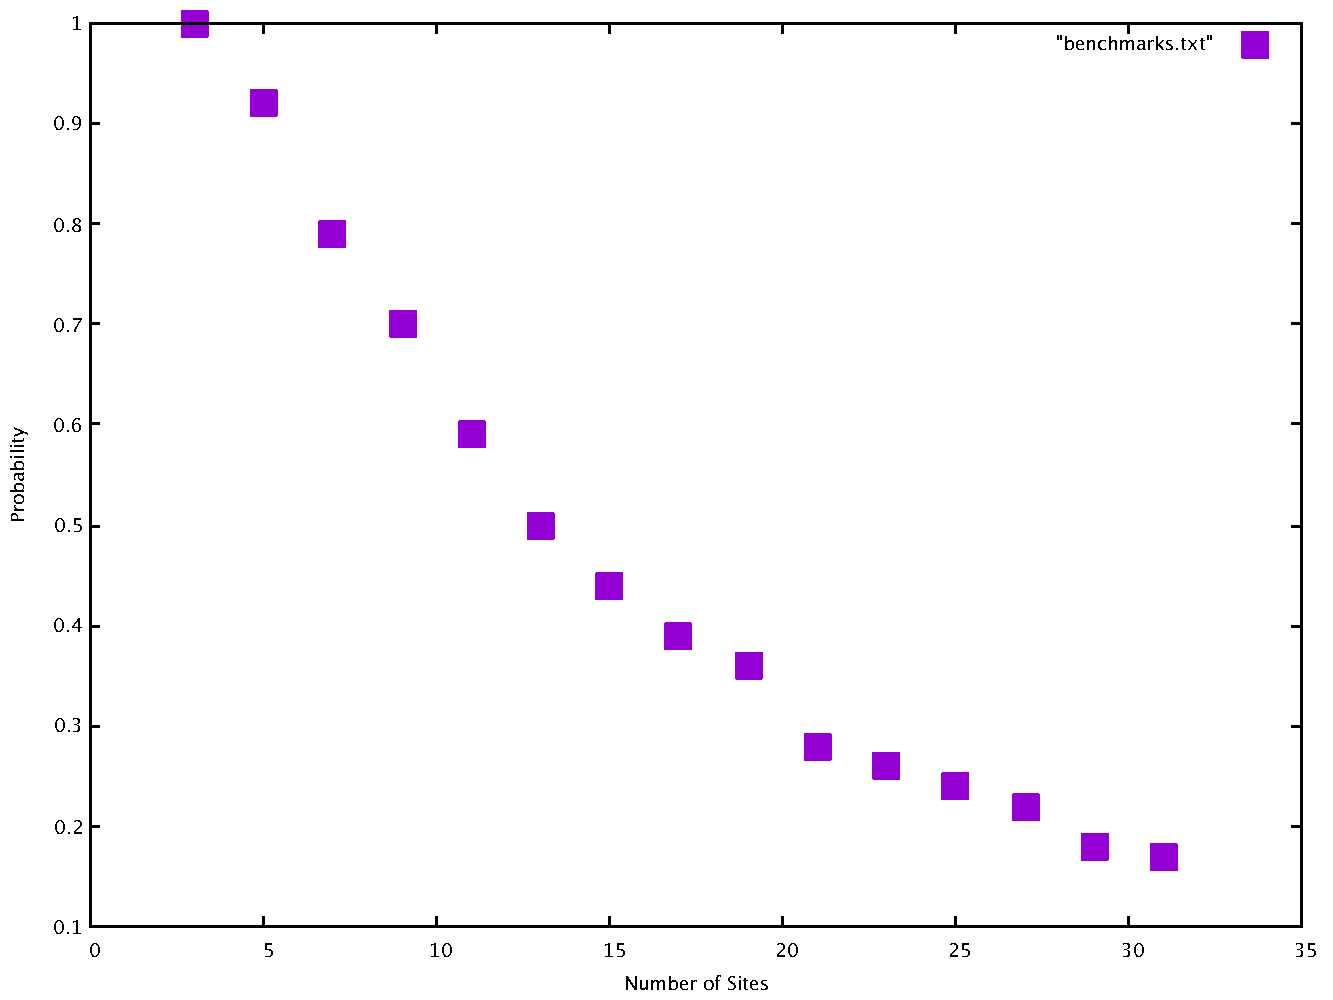
\includegraphics[width=10cm]{./figures/benchmarks.pdf}
\caption{Time Independent Benchmarks up to N=31}
\end{figure}

It is clear that the time-independent algorithm does indeed not work, as we expected. The probability decreases as the number of sites N increases, \red{I noticed that for large N the probability (fixing $\gamma$) converges to $p=0.1$. Further investigation is needed.}

\subsubsection{\textbf{Time-Dependent Algorithm}}
We then considered the time-dependent hamiltonian introduced in Section ?, and following the \textit{probability grid evaluation} procedure discussed before we computed the probability. Given the computational efficency over the regular $\beta$-T optimization we were able to compute results up to N = 71, although from 31 to 71 only the 1st and 7th (e.g. 41,47) were calculated. \\ \\
It is however clear that the grid-evaluation approach does not produce unique values of $(T,\beta)$ corrisponding to the absolute probability maximum. On the other hand is able to give a qualitative idea on the probability distribution for various $(T,\beta)$ combinations. We then present the found data with a \textbf{heatmap plot} such the one below, which makes quite easy to visualize the result.
\begin{figure}[ht]
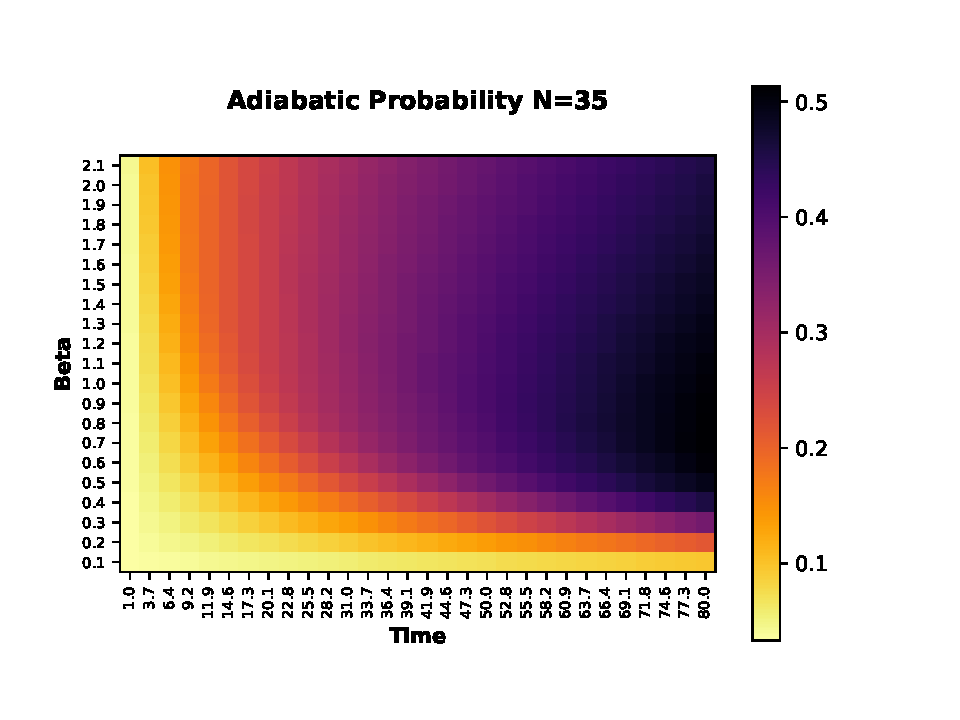
\includegraphics[width=10cm]{./figures/example.pdf}%
\caption{Time Dependent heatmap example, N=35}
\end{figure}

The task now is two develop a method to compare the time-independent and time-dependent algorithms. We first naively look at a qualitative comparison that immediately shows that the time-dependent algorithm is able to find higher probabilities but at the expense of worst time scaling; secondly we introduce a quantity to compare the two methods numerically.

\subsubsection{\textbf{Qualitative Comparison}}
In order to qualitatively compare the two approaches to quantum search we will consider a heatmap plot where we superimpose probability \textbf{contour lines} corrisponding to the following probability (and with the following format):
\begin{itemize}
  \item (solid) p = 0.99, p = 0.95, p = 0.90 for the time-dependent results
  \item (dashed) the probability found in the corrisponding time-independent results
\end{itemize}
These, with the corrisponding time T at which the time-independent probability is found (given by a vertical line), should give a qualitative method to compare the two approaches. How shall we do so?
\begin{itemize}
	\item Look for any intersection between the dashed contour line and the vertical line
	\item If it does intersect the intersection point(s) represent a $(\gamma, T)$ combination that is equivalent as the time-independent algorithm in terms of probability
	\item If the dashed contour line and the vertical line identify a bounded region (\red{might be necessary a figure to explain this}), that particular region represents a $(\gamma, T)$-space for which the time-dependent algorithm performs better than the time-independent one.
\end{itemize}


\begin{figure}[ht]
\begin{tabular}{cc}
  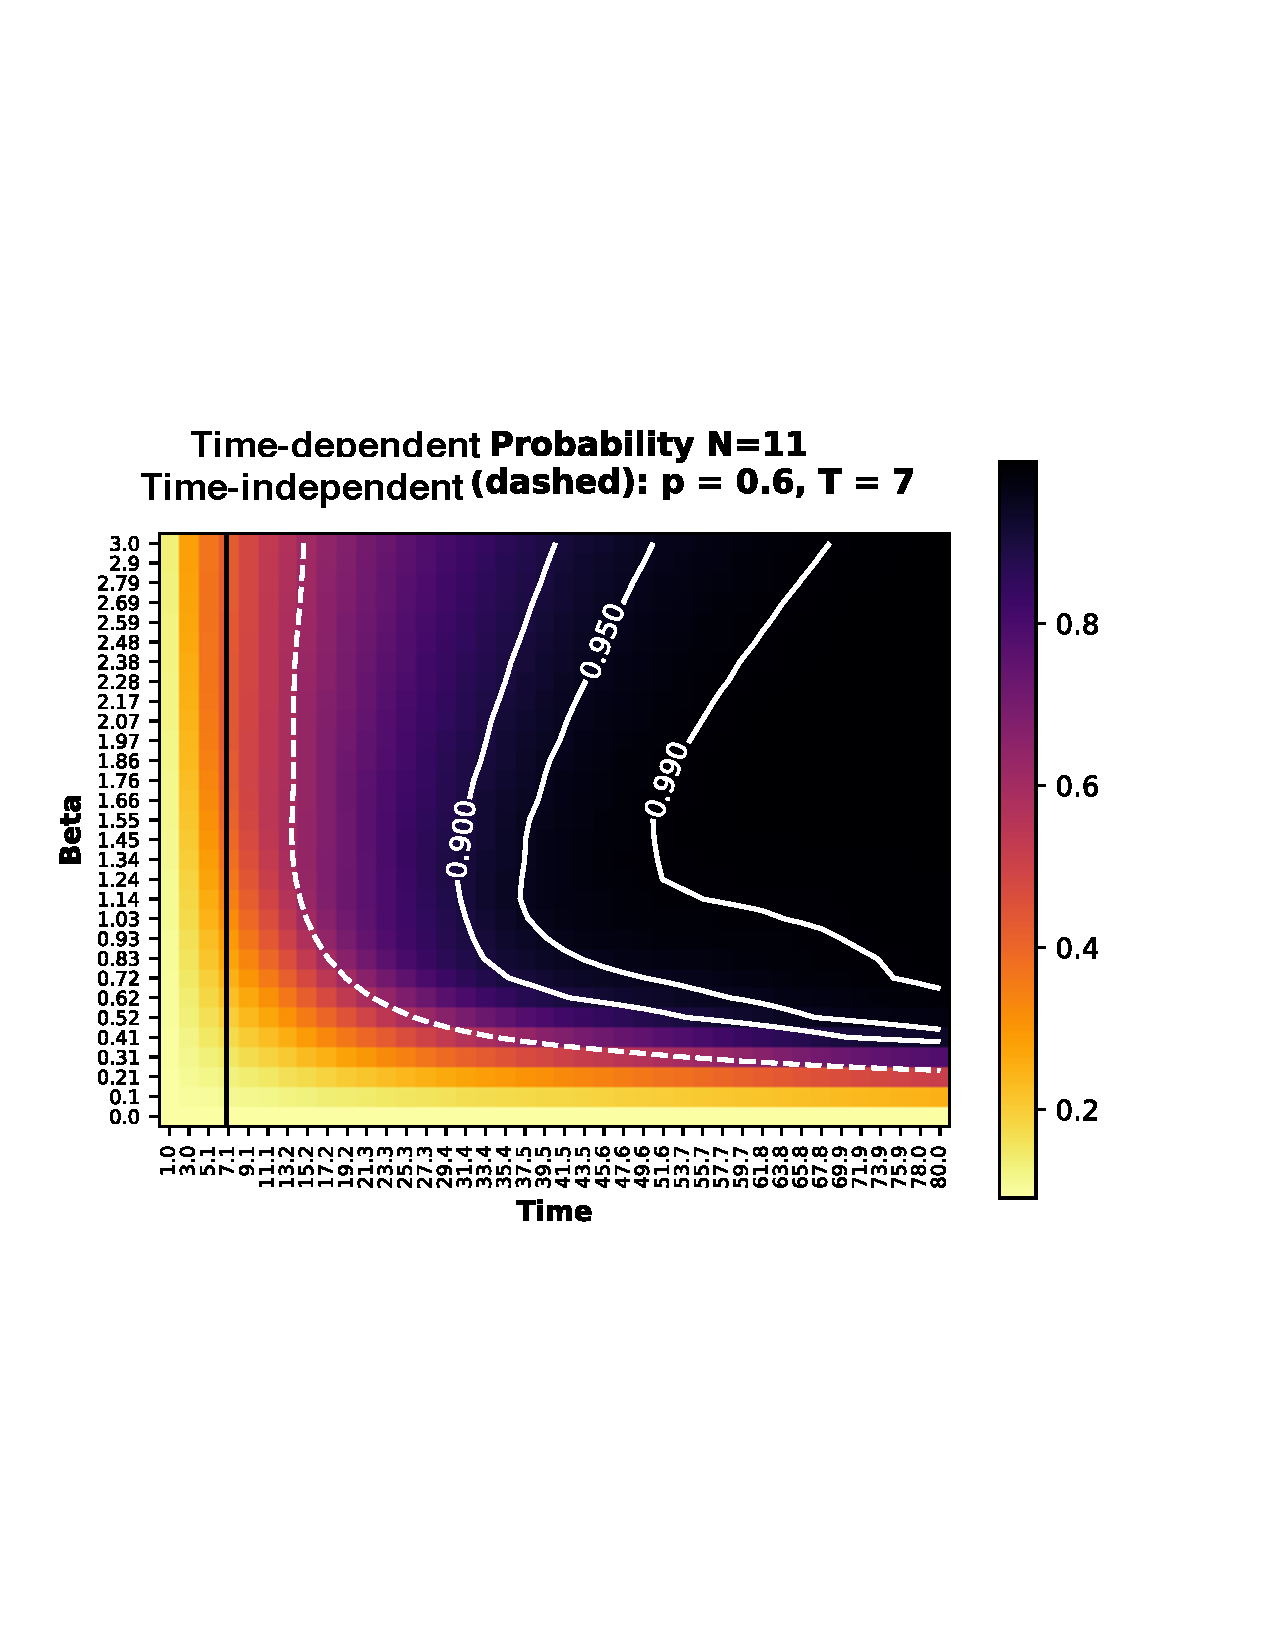
\includegraphics[width=90mm]{./figures/11.pdf} &   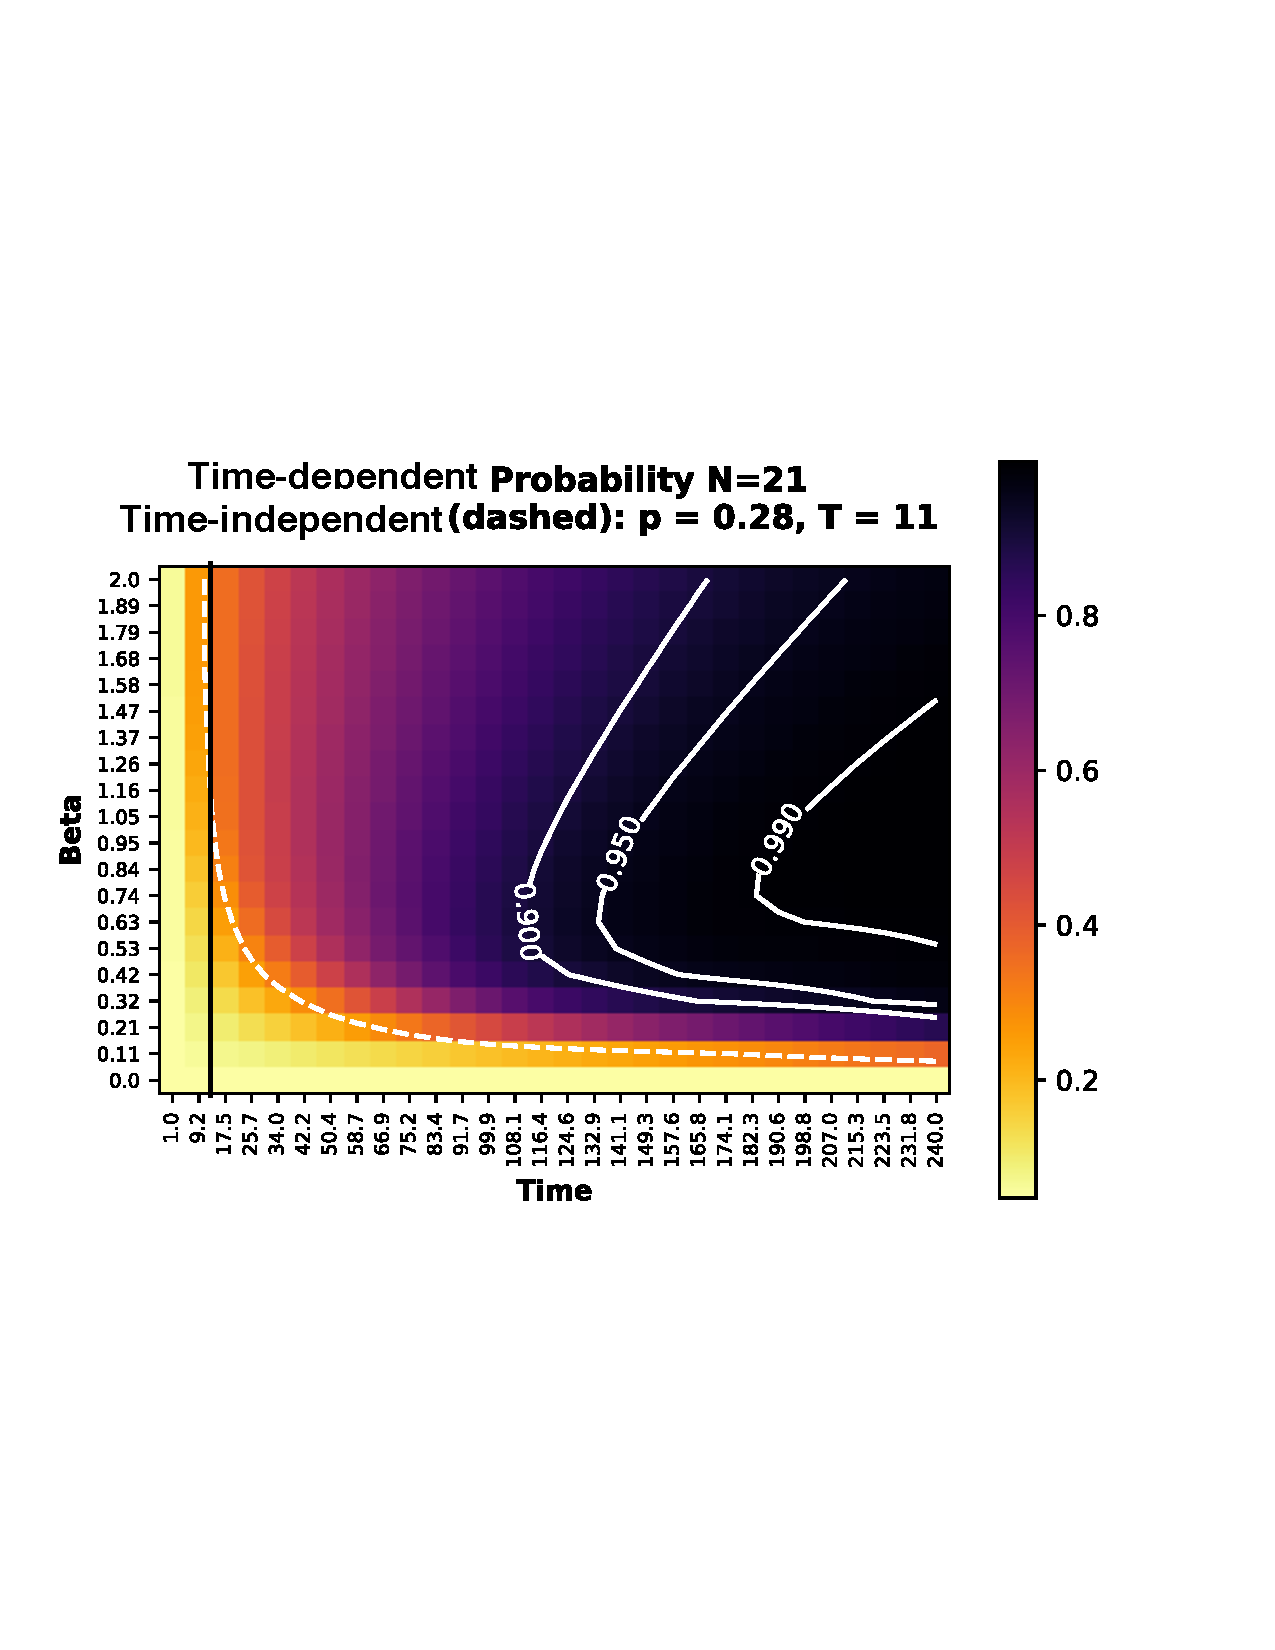
\includegraphics[width=90mm]{./figures/21.pdf} \\
(a) N = 11 & (b) N = 21\\[6pt]
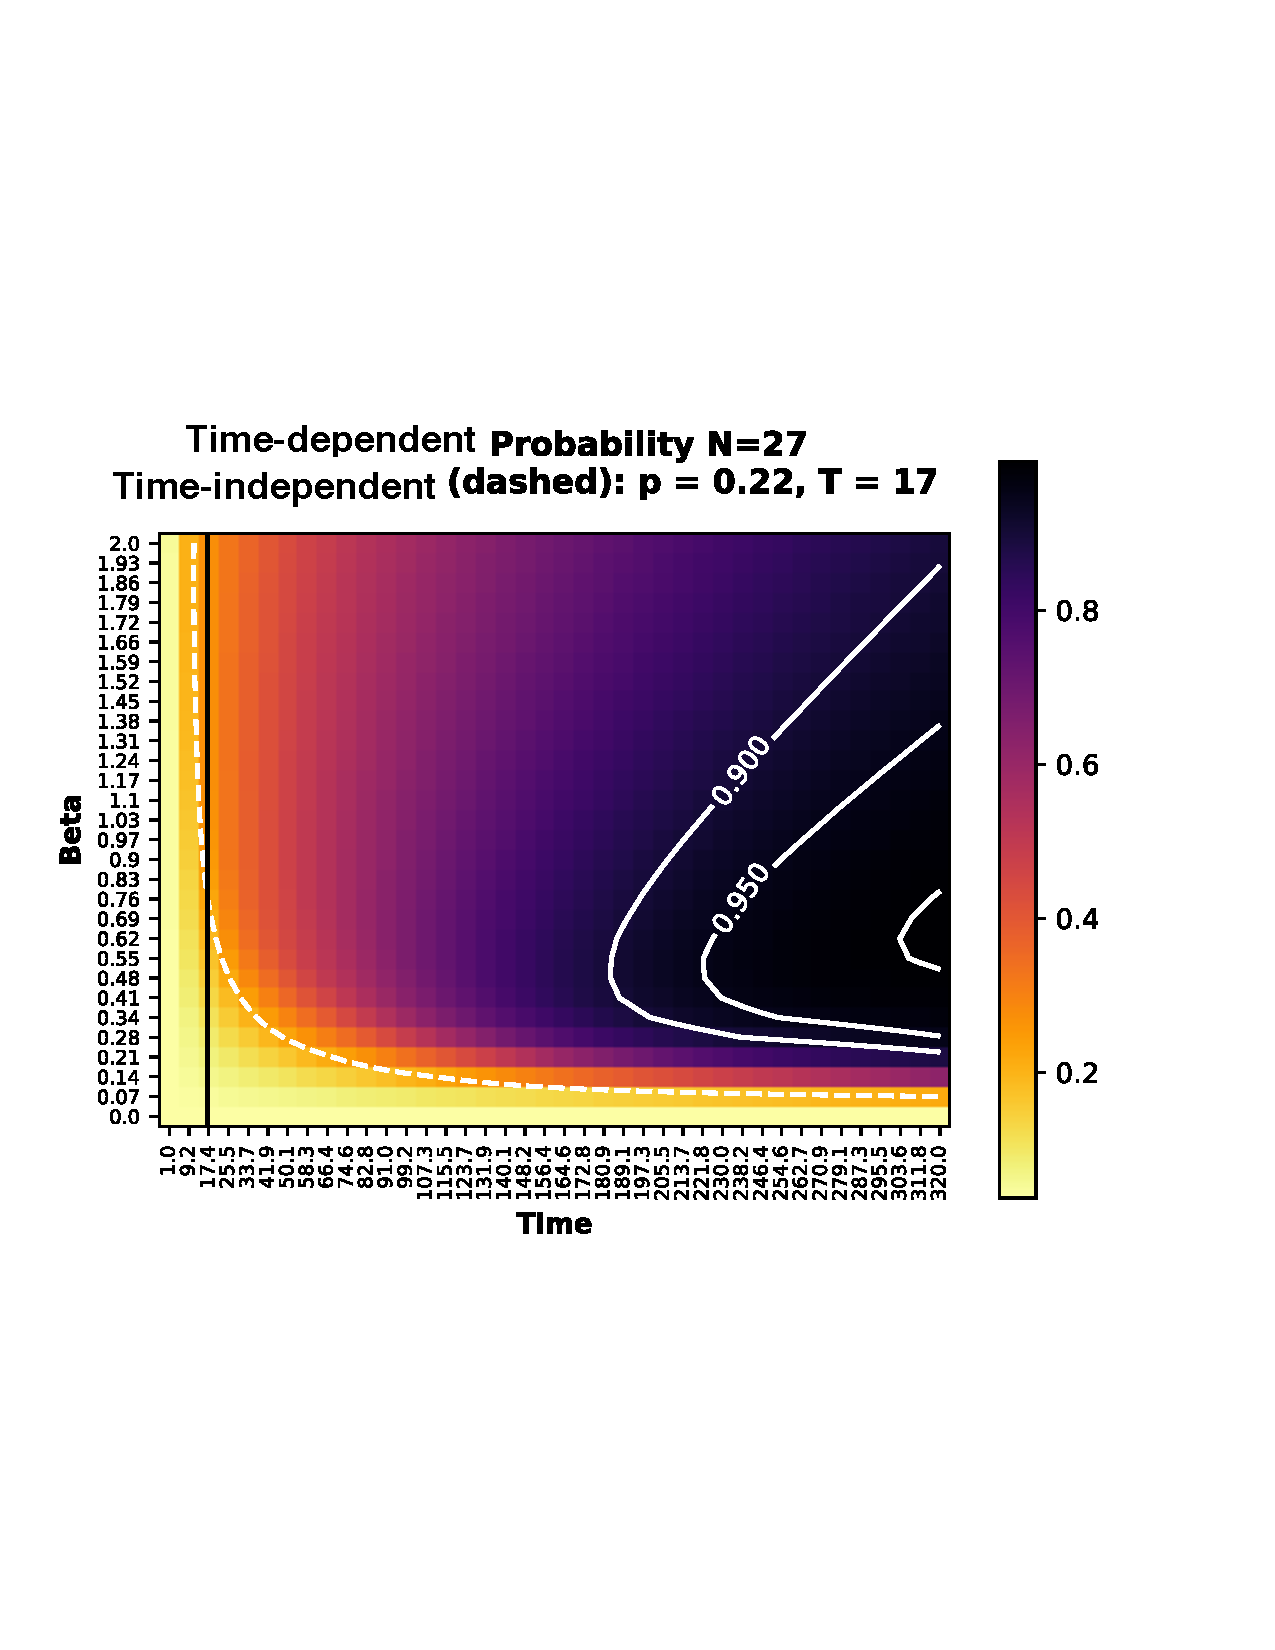
\includegraphics[width=90mm]{./figures/27.pdf} &   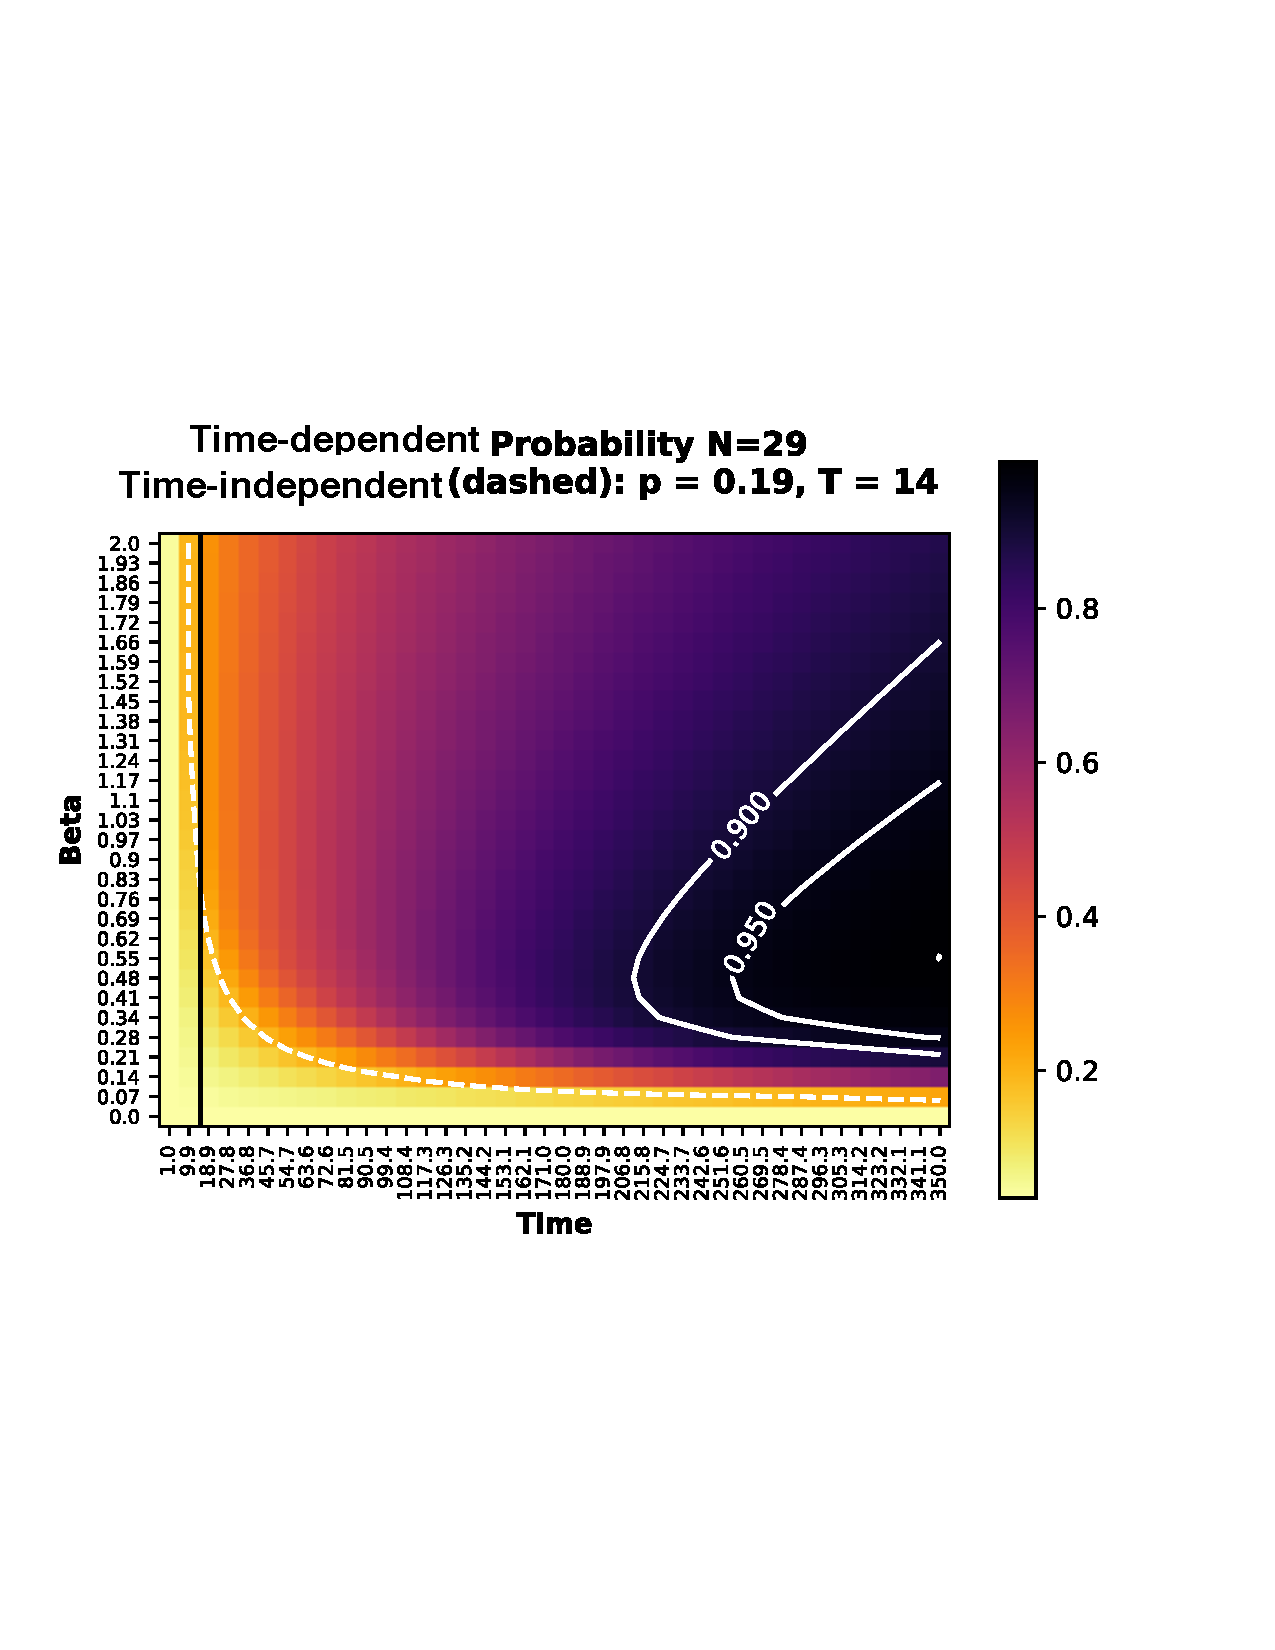
\includegraphics[width=90mm]{./figures/29.pdf} \\
(c) N = 27 & (d) N = 29\\[6pt]
\end{tabular}
\end{figure}

%\clearpage

\subsubsection{\textbf{Numerical Comparison}}
In order to numerically compare the two approaches we define a quantity $\delta$ in the following way:
\begin{equation}
  \delta = \min\Big(\frac{T}{p}\Big)
\end{equation}
The quantity T/p represents the total time necessary to get to unitary probability. Finding the minimum of that quantity corresponds to finding the best combination of T and p that gets to unity with the minimum T. \\ \\
What we do is thus for each vertical column of the grid, i.e. constant T and variable $\beta$, computing the maximum probability and finding the quantity T/p. We than find the minimum of all the T/p calculated. In this way we \textbf{reduce a grid to a single value} to compare to the time-independent results. \\ \\
The following plot compares the time-independent approach to the time-dependent one, using for the first the quantity T/p evaluated with the \textit{$\beta$-T optimized} probability while the latter uses the quantity $\delta$. \\

\begin{figure}[ht]
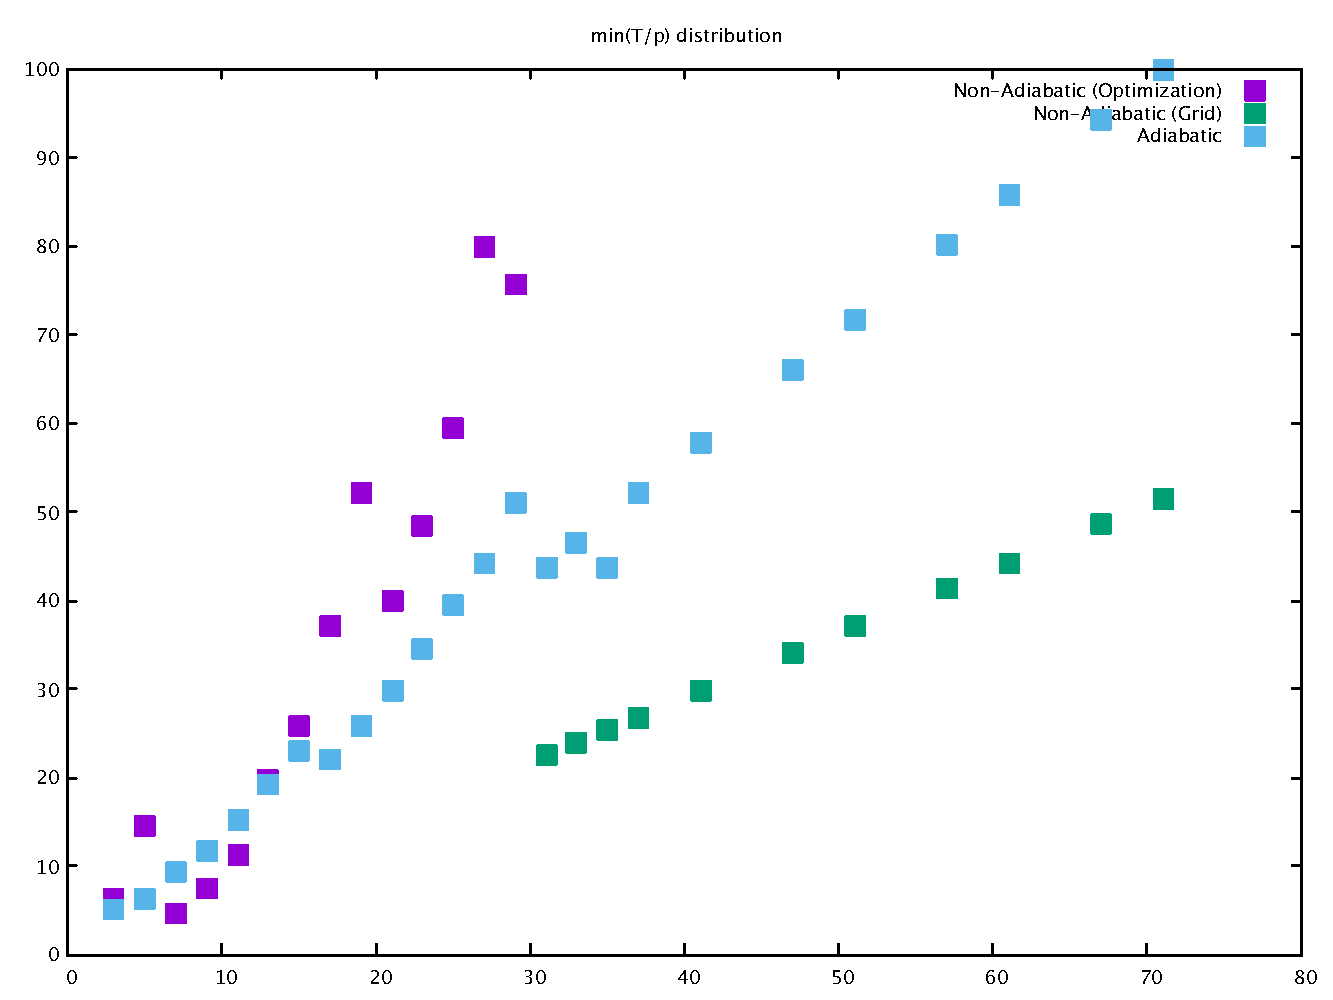
\includegraphics[width=9cm]{./figures/delta.pdf}%
\caption{\textbf{$\delta$ values comparing methods:} the figure shows the distribution of the delta-quantity for the time-dependent hamiltonian (light blue), the time-independent hamiltonian with $\gamma-T$ optimization (purple) and the time-independent hamiltonian with the grid evaluation (green)}
\end{figure}
\red{It's necessary to decide whether to use the grid evaluation approach or the $\gamma-T$ optimization. It is indeed clear that the two produce two drastically different results. In additions comments on the fact that a lower bound on T might be needed in order to get interesting results on delta.}

\subsubsection{\textbf{Different s(t) shapes}}
As we introduced in Section III we're interested in determining how influencial is the shape of s(t) in the probability distribution. We then proceed as in Section ? using the step function s(t) previously discussed. \\ To compare we consider the quantity $\delta$. Since we're interested in the trend for large N we ignore small N and only consider a few sampled N between 35-70.

\begin{figure}[ht]
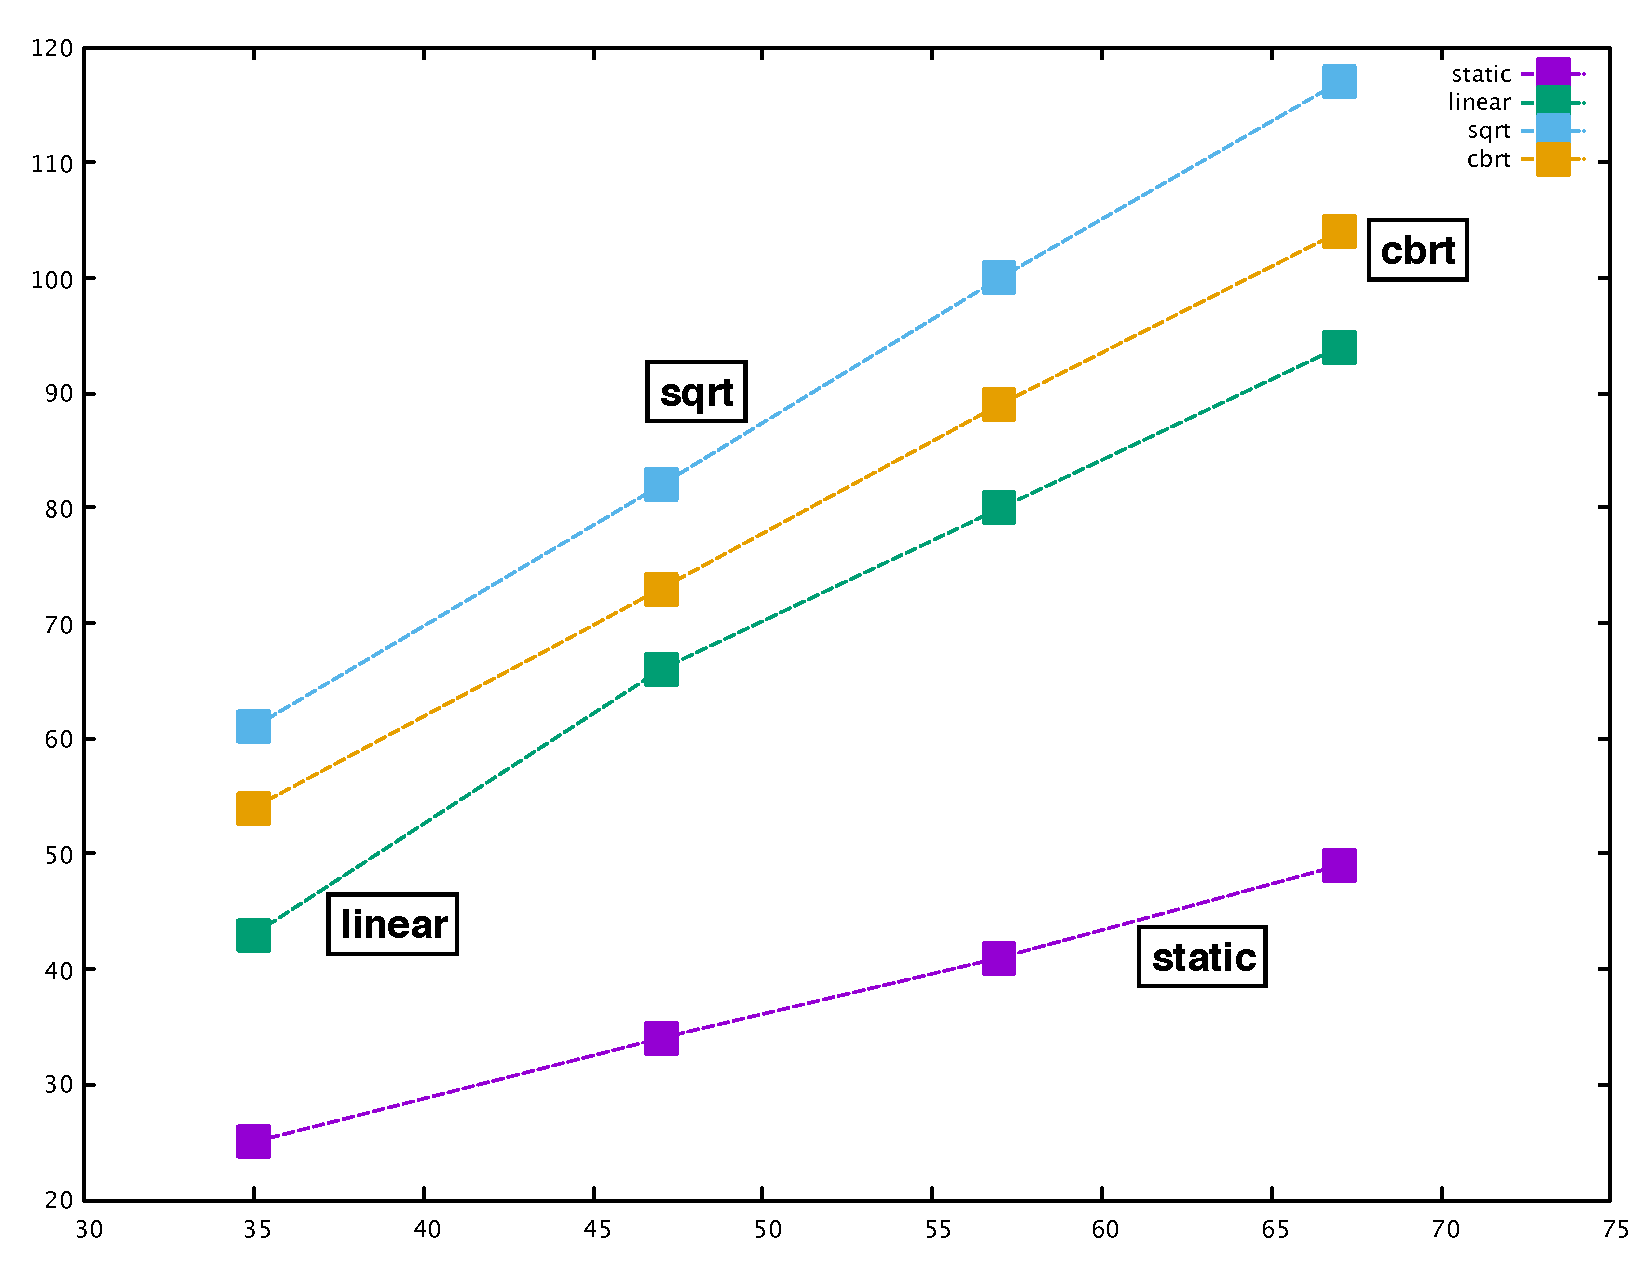
\includegraphics[width=8cm]{./figures/s(t).pdf}
\caption{Delta distrubution for different s(t). Computed for N = 35,47,57,67}
\end{figure}

As the plot shows however we do not see any speedup for functions that are not linear, on the contrary we do get poorer results. The time-independent implementation remains the best performing one, followed by linear, cubic root and square root.

\subsubsection{\textbf{Localization}}
We can clearly see from the heatmap plots that for large T the probabability gets bigger, and it will eventually get to one. This is, as we already mentioned, a direct consequence of the adiabatic theorem. \\ A further analysis is due, focusing on studying the probability distribution with a more quantitative approach. That being said the localization is a key feature of the time-dependent approach to quantum search.

\subsection{Complete graph}
\red{This section should include a comparison between time dependent and time independent approach to quantum search for the complete graph. We're interested in benchmarks to compare to the circular graph. For now the results we have are partial and yet not enough to show what we want\\ It might also be interesting looking into the order of the probability for p=0.9.}
%%%%%%%
%FUTURE DEVELOPMENTS
%%%%%%%
\section{Future Developments}
Follows a list of things to be done
\begin{itemize}
	\item Benchmarks for the complete graph
	\item Comments on s(t), more in-depth description (and Adiabatic Theorem consideration)
	\item Additional results for s(t), also using the one introduced by Cerf
	\item Comments on heatmap and computational time
	\item Grover's quantum search
	\item Search on complete graph (analitical solution)
	\item Additional parameters for the discussion on the optimization algorithm and the ode solver
	\item Better figures!
	\item Decide which method to use for the time-independent delta values
	\item In the qualitative comparison the vertical T-line is not very effective in showing what I wanted

\end{itemize}
\clearpage
%%%%%%%
%APPENDIX
%%%%%%%


\section{Appendix}
In this section an overview of the computational methods is presented, focusing the attention on the \textbf{optimization algorithm} and the \textbf{differential equation solver}. Additionally the normalization error is discussed. Lastly computational reasoning for the \textbf{probability grid evaluation} are presented. \\

Most all numerical simulations were performed using \textbf{Python}. Numerical methods such as optimization and ODE Solver come directly from python's native \textbf{Scipy}. In addition, a CPU-multiprocessing library, \textbf{Ray}, has been used to speed up the grid probability evaluation quite noticeably. Heatmap plots were created using python matplotlib, while additional plots were created with gnuplot.

\subsection{Optimization Algorithm}
In Section III a series of benchmark were performed to compare the time-dependent and time independent hamiltonian approach to the search problem. In order to determine which optimization algorithm fitted the best for the task, a number of possible algorithm were tested, such as \textit{shgo, dualannealing, minimize, LHSBH} and \textit{Basin-Hopping}.\\ \\
Due to the oscillating nature of the probability (\red{a figure is needed}) the scipy native \textbf{Basinhopping algorithm} was used. As the name suggests the algorithm performs a series of randomized hops, i.e. jumps, of the coordinates in order to find the true maximum This fits particularly well with the series of maxima and minima of the probability function (for fixed $\gamma$) in the time-independent hamiltonian. \\\red{Additional information on the parameter used are needed (e.g. step size, number of iterations)}

\subsection{Schroedinger Solver and Normalization Error}
In Section II we presented an evolution which is governed by a time-dependent hamiltonian, used to find the evolved state $|\psi(t)\rangle$. This is accomplished by solving the usual Schroedinger equation using Scipy's \textbf{integrate.solve\_ivp}, that provides a wide varieties of integrations methods. \\

As it's routine we used Runge-Kutta RK45, which as stated in the documentation it's a explicit Runge Kutta method of order 4(5). The error is controlled assuming fourth order accuracy, but steps are taken using the fifth-order accurate formula. In addition, the integrator is adaptive, meaning that the time step is chosen for optimal error control. Regarding the error, the algorithm provides two distinct parameters to set a targeted limit, namely the \textbf{relative (rtol)} and \textbf{absolute tolerances (atol)}. The first provides a relative accuracy, i.e. the number of digits, while the latter is used to keep the local error estimate below the threshold \textit{atol + rtol*abs(y)}. Determining the correct combinations of the two parameters is key for achieving the desired error. A few of those are presented in the following table, where a worst case scenario (N=101, T=1000) is used and the error is evaluated on the expected normalized state. The combination of rtol and atol bolded is the one we used in the solver, which gives us a small enough error on the normalization without greater computational expense.\\

\begin{figure}[ht]
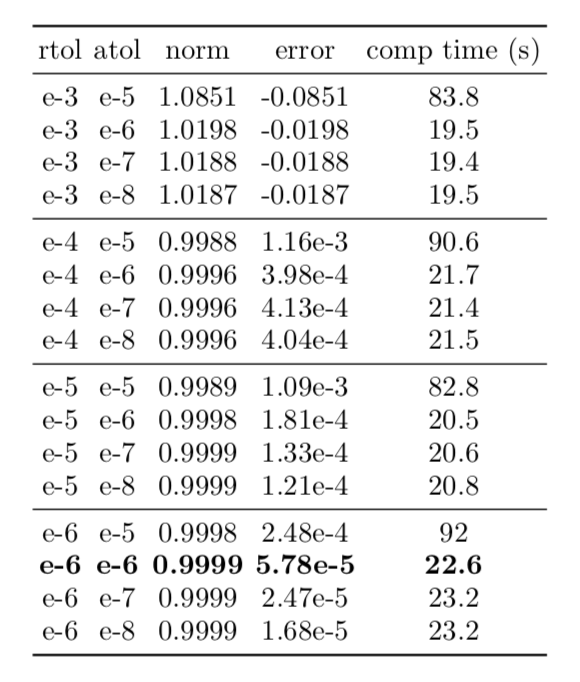
\includegraphics[width=5cm]{./figures/runge.png}%
\end{figure}

\clearpage
%\begin{center}
%\begin{adjustbox}{width=6cm}
%\begin{tabular}{>{\rowmac}c>{\rowmac}c>{\rowmac}c>{\rowmac}c>{\rowmac}c<{\clearrow}} \toprule
%    {rtol} & {atol} & {norm} &{error} & {comp time (s)}\\ \midrule
%    e-3  & e-5 & 1.0851 & -0.0851 & 83.8\\
%    e-3  & e-6 & 1.0198 & -0.0198 & 19.5\\
%    e-3  & e-7 & 1.0188 & -0.0188 & 19.4\\
%    e-3  & e-8 & 1.0187 & -0.0187 & 19.5\\ \midrule

%    e-4  & e-5 & 0.9988 & 1.16e-3 & 90.6\\
%    e-4  & e-6 & 0.9996 & 3.98e-4 & 21.7\\
%    e-4  & e-7 & 0.9996 & 4.13e-4 & 21.4 \\
%    e-4  & e-8 & 0.9996 & 4.04e-4 & 21.5 \\ \midrule

%    e-5  & e-5 & 0.9989 & 1.09e-3 & 82.8\\
%    e-5  & e-6 & 0.9998 & 1.81e-4 & 20.5\\
%    e-5  & e-7 & 0.9999 & 1.33e-4 & 20.6\\
%    e-5  & e-8 & 0.9999 & 1.21e-4 & 20.8\\ \midrule

%  e-6  & e-5 & 0.9998 & 2.48e-4 & 92  \\
%    \setrow{\bfseries} e-6  & e-6 & 0.9999 & 5.78e-5 & 22.6\\
%    e-6  & e-7 & 0.9999 & 2.47e-5 & 23.2\\
%    e-6  & e-8 & 0.9999 & 1.68e-5 & 23.2\\ \bottomrule

%\end{tabular}
%\end{adjustbox}
%\end{center}

\end{document}
